\subsection{Суммарный выходящий поток RQ--системы} \label{section_simple_summary}
Суммарный выходящий поток RQ--системы подразумевает, что приходящие заявки и заявки, вызываемые прибором самостоятельно, являются однородными, посему результат работы системы рассматривается как совокупность обслуженных заявок входящего потока и вызванных. 
\begin{figure}[H]
	\centering
	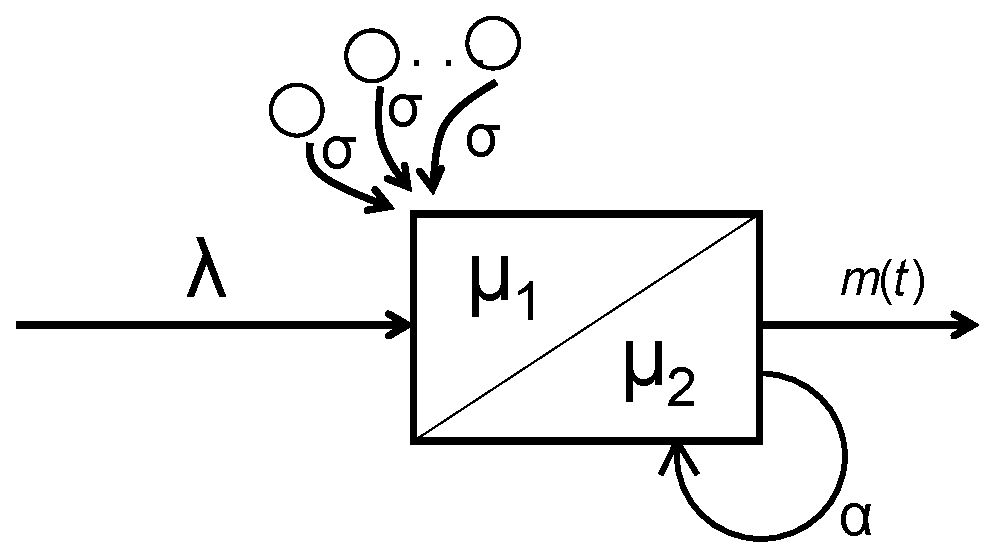
\includegraphics[scale=0.5]{summary_output_model.eps}
	\caption{Модель RQ--системы с суммарным выходящим потоком}
	\label{summary_output_model_fig}
\end{figure}
Введем обозначение: $m_(t)$ --- число обслуженных заявок в момент времени $t$.


\subsubsection{Уравнения Колмогорова}
Итак, мы имеем три характеристики, определяющие результат функционирования системы за некоторое время $t$: состояние прибора --- $k(t)$, количество заявок на орбите --- $i(t)$ и количество обслуженных заявок --- $m(t)$, что можно представить в виде трехмерного Марковского процесса
\begin{equation*}
	\{k(t),i(t),m(t)\}.
\end{equation*}

Заметим, что именно такая комбинация характеристик будет являться Марковским процессом, так как даёт достаточно информации о том, какое состояние система примет в следующий момент времени. Для этого необходимо знать, в каком состоянии прибор был в предшествующий момент времени, и какое количество заявок находилось в источнике повторных вызовов.
Следующее состояние, которое прибор может принять, зависит от состояния, в котором он находился прежде, то есть, каждое из трех состояний $k(t)$ принимается прибором с некоторыми вероятностями. Введем их в рассмотрение
\begin{equation*}
	\begin{split}
		P\{k(t)=0,i(t)=i,m(t)=m\} &=P_{0}(i,m,t),\\
		P\{k(t)=1,i(t)=i,m(t)=m\} &=P_{1}(i,m,t),\\
		P\{k(t)=2,i(t)=i,m(t)=m\} &=P_{2}(i,m,t).
	\end{split}
\end{equation*}

Теперь, необходимо определить вероятность перехода в каждое из трех состояний. Для этого обратимся к модели и рассмотрим $k(t) = 0$, то есть, состояние, в котором прибор свободен. Чтобы в следующий момент времени $t+\Delta t$ прибор был свободен необходимо выполнение одного из следующих условий:
\begin{enumerate}
	\item Прибор был свободным в момент времени $t$ и к моменту времени $t+\Delta t$  прибор не вызвал заявку, не пришла заявка с входящего потока и не было обращений заявок с орбиты.
	\item На момент времени $t+\Delta t$ прибор закончил обслуживание заявки с входящего потока.
	\item На момент времени $t+\Delta t$ прибор закончил обслуживание вызываемой заявки.
\end{enumerate}
Таким образом, применяя формулу полной вероятности, вероятность того, что прибор окажется свободен в момент времени $t+\Delta t$, равна сумме вероятностей наступления вышеперечисленных условий:
\begin{equation*}
	\begin{split}
	P_{0}(i,m,t+\Delta t) &=P_{0}(i,m,t)(1-\alpha\Delta t)(1 - i\sigma\Delta t)(1-\lambda\Delta t)+ \\ &+ P_{1}(i,m-1,t)\mu_{1}\Delta t + P_{2}(i,m-1,t)\mu_{2}\Delta t.
	\end{split}
\end{equation*}

Аналогично, для принятия состояния, в котором прибор занят, необходимо выполнение одного из следующих условий:
\begin{enumerate}
	\item Прибор был занят в момент времени $t$,  и к моменту времени $t+\Delta t$ прибор не закончил обслуживание заявки, и не пришла заявка с входящего потока.
	\item Прибор был свободен, и пришла заявка с входящего потока.
	\item Прибор был свободен, и повторно обратилась заявка с орбиты.
	\item Прибор был занят, и пришла заявка с входящего потока, сразу переместившись на орбиту.
\end{enumerate}
В результате получим следующее равенство:
\begin{equation*}
	\begin{split}
			P_{1}(i,m,t+\Delta t)&=P_{1}(i,m,t)(1-\lambda\Delta t)(1-\mu_{1}\lambda\Delta t)+P_{0}(i,m,t)\lambda\Delta t +\\ &+ P_{0}(i+1,m,t)(i+1)\sigma\Delta t + P_{1}(i-1,m,t)\lambda\Delta t + o(t).
	\end{split}
\end{equation*}

Вероятность принятия прибором состояния обслуживания вызываемой заявки является суммой следующих вероятностей:
\begin{enumerate}
	\item Прибор обслуживал вызываемую заявку и к моменту времени $t+\Delta t$ не закончил ее обслуживание, и не пришла заявка с входящего потока.
	\item Прибор обслуживал вызываемую заявку, и пришла заявка с входящего потока. Поскольку прибор занят, она ушла на орбиту.
	\item Прибор был свободен, и он вызвал заявку.
\end{enumerate}
Получим равенство:
\begin{equation*}
	\begin{split}
	P_{2}(i,m,t+\Delta t) &=P_{2}(i,m,t)(1-\alpha\Delta t)(1 - \lambda\Delta t)(1 - \mu_{2}\Delta t)+ \\ &+ P_{2}(i-1,m,t)\lambda\Delta t + P_{0}(i,m,t)\alpha\Delta t + o(t).
\end{split}
\end{equation*}

Запишем получившуюся систему уравнений
\begin{equation*} 
	\begin{split}
		P_{0}(i,m,t+\Delta t)&=P_{0}(i,m,t)(1-\alpha\Delta t)(1 - i\sigma\Delta t)(1-\lambda\Delta t) +\\ &+ P_{1}(i,m-1,t)\mu_{1}\Delta t + P_{2}(i,m-1,t)\mu_{2}\Delta t,
		\\
		P_{1}(i,m,t+\Delta t)&=P_{1}(i,m,t)(1-\lambda\Delta t)(1-\mu_{1}\lambda\Delta t)+P_{0}(i,m,t)\lambda\Delta t +\\ &+ P_{0}(i+1,m,t)(i+1)\sigma\Delta t + P_{1}(i-1,m,t)\lambda\Delta t + o(t),
		\\
		P_{2}(i,m,t+\Delta t)&=P_{2}(i,m,t)(1-\alpha\Delta t)(1 - \lambda\Delta t)(1 - \mu_{2}\Delta t) +\\ &+ P_{2}(i-1,m,t)\lambda\Delta t + P_{0}(i,m,t)\alpha\Delta t + o(t).
	\end{split}
\end{equation*}
Так как все слагаемые содержат $\Delta t$, разделим систему на $\Delta t$ и сделаем предельный переход $\Delta t \rightarrow 0$
\begin{equation} \label{kolmogorov_equations_summary}
	\begin{split}
		\frac{{\partial P_{0}(i,m,t)}}{{\partial t}} &= -(\lambda + i\sigma + \alpha)P_{0}(i,m,t) + P_{1}(i,m-1,t)\mu_{1} + P_{2}(i,m-1,t)\mu_{2},
		\\
		\frac{{\partial P_{1}(i,m,t)}}{{\partial t}} &= -(\lambda + \mu_{1})P_{1}(i,m,t) + (i+1)\sigma P_{0}(i+1,m,t) + \lambda  P_{0}(i,m,t),
		\\
		\frac{{\partial P_{2}(i,m,t)}}{{\partial t}} &= -(\lambda + \mu_{2})P_{2}(i,m,t) + \lambda P_{2}(i-1,m,t) + \alpha  P_{0}(i,m,t).
	\end{split}
\end{equation}	

Полученная система уравнений --- система дифференциальных уравнений Колмогорова, где в левой части каждого уравнения находится производная вероятности состояния рассматриваемого процесса, а в правой --- сумма произведений вероятностей состояний, из которых прибор может принять это состояние, на интенсивности соответствующих потоков заявок. Решением данной системы будут являться вероятности всех состояний прибора в виде функций времени. Таким образом, задача сводится к решению данной системы дифференциальных уравнений.

Решить данную систему аналитически не получится, так как это система бесконечного числа дифференциальных конечно--разностных уравнений с переменными коэффициентами. 
Для того, чтобы перейти к конечному числу уравнений, введем частные характеристические функции, обозначив $j=\sqrt{-1}$,
\begin{equation*}
	H_{k}(u_{1},u,t) = \sum_{i=0}^{\infty}
	\sum_{m=0}^{\infty}  
	e^{ju_{1}i}e^{jum} P_{k}(i,m,t).
\end{equation*}
Тогда перепишем систему \eqref{kolmogorov_equations_summary} в виде
\begin{equation} \label{characteristic_equations_summary}
	\begin{split}
		\frac{{\partial H_{0}(u_{1},u,t)}}{{\partial t}} &= -(\lambda + \alpha)H_{0}(u_{1},u,t) + j\sigma
		\frac{{\partial H_{0}(u_{1},u,t)}}{{\partial u_{1}}} +\\  &+ \mu_{1} e^{ju}H_{1}(u_{1},u,t) + \mu_{2}e^{ju}H_{2}(u_{1},u,t) ,
		\\
		\frac{{\partial H_{1}(u_{1},u,t)}}{{\partial t}} &= -(\lambda + \mu_{1})H_{1}(u_{1},u,t) - j\sigma e^{-ju_{1}}
		\frac{{\partial H_{0}(u_{1},u,t)}}{{\partial u_{1}}} +\\  &+ \lambda H_{0}(u_{1},u,t) + \lambda e^{ju_{1}}H_{1}(u_{1},u,t) ,
		\\
		\frac{{\partial H_{2}(u_{1},u,t)}}{{\partial t}} &= -(\lambda + \mu_{2})H_{2}(u_{1},u,t)  + \lambda e^{ju_{1}}H_{2}(u_{1},u,t) +\\  &+ \alpha H_{0}(u_{1},u,t).
	\end{split}
\end{equation}  

Таким образом, мы получили ровно три дифференциальных уравнения в частных производных с переменными коэффициентами.
\subsubsection{Метод асимптотического анализа}
Полученную систему дифференциальных уравнений в частных производных \eqref{characteristic_equations_summary} будем решать методом асимптотического анализа \cite{nazarov2017asymptotic} в предельном условии большой задержки заявок на орбите ($\sigma \rightarrow 0$).
Обозначим $\epsilon = \sigma,   u_{1}= \epsilon w,   F_{k}(w,u,t,\epsilon) = H_{k}(u_{1},u,t)$, тогда система запишется в виде
\begin{equation} \label{asymptotic_equations_summary}
	\begin{split}
		\frac{{\partial F_{0}(w,u,t,\epsilon)}}{{\partial t}} &= -(\lambda + \alpha)F_{0}(w,u,t,\epsilon) + j
		\frac{{\partial F_{0}(w,u,t,\epsilon)}}{{\partial w}} +\\  &+ \mu_{1} e^{ju}F_{1}(w,u,t,\epsilon) + \mu_{2}e^{ju}F_{2}(w,u,t,\epsilon) ,
		\\
		\frac{{\partial F_{1}(w,u,t,\epsilon)}}{{\partial t}} &= -(\lambda + \mu_{1})F_{1}(w,u,t,\epsilon) - j e^{-j\epsilon w}
		\frac{{\partial F_{0}(w,u,t,\epsilon)}}{{\partial w}} +\\  &+ \lambda F_{0}(w,u,t,\epsilon) + \lambda e^{j\epsilon w}F_{1}(w,u,t,\epsilon) ,
		\\
		\frac{{\partial F_{2}(w,u,t,\epsilon)}}{{\partial t}} &= -(\lambda + \mu_{2})F_{2}(w,u,t,\epsilon)  + \lambda e^{j\epsilon w}F_{2}(w,u,t,\epsilon) +\\  &+ \alpha F_{0}(w,u,t,\epsilon).
	\end{split}
\end{equation}  

С помощью введенных функций можно записать характеристическую функцию процесса $m(t)$ в следующем виде
\begin{equation*}
	M\{\exp(jum(t))\}=\sum_{k=0}^{2}H_{k}(0,u_{1},u_{2},t) = \sum_{k=0}^{2}F_{k}(0,u_{1},u_{2},t,\epsilon).
\end{equation*}

\begin{theorem}
	Асимптотические приближение характеристической функции числа обслуженных заявок за некоторое время $t$ имеет вид
	\begin{equation*} \label{theorem_summary}
		\begin{split}
			\lim_{\sigma \xrightarrow{} 0} M\{\exp(jum(t))\} &= \lim_{\epsilon \xrightarrow{} 0} \sum_{k=0}^{2}F_{k}(0,u,t,\epsilon) = \boldsymbol{R} \cdot \exp\{G(u)t\} \cdot \boldsymbol{E},
		\end{split}
	\end{equation*}
	где 
	\begin{equation*}
		\boldsymbol{G}(u)=\begin{bmatrix}
			-(\lambda + \alpha + \kappa) & \mu_{1}e^{ju} &  \mu_{2}e^{ju}\\
			\kappa+\lambda & -\mu_{1} & 0\\
			\alpha & 	0 &	-\mu_{2}
		\end{bmatrix}^{T},
	\end{equation*}
	вектор--строка $\boldsymbol{R}=\{R_{0},R_{1},R_{2}\}$ --- стационарное распределение вероятности состояния прибора
	\begin{equation*}
		\boldsymbol{R}=\left\{\frac{\mu_{2}(\mu_{1} - \lambda)}{\mu_{1}(\mu_{2} - \alpha)},\frac{\lambda}{\mu_{1}},\frac{\alpha(\mu_{1} - \lambda)}{\mu_{1}(\mu_{2} + \alpha)}\right\},
	\end{equation*}
	$\kappa$ --- нормированное среднее число заявок на орбите
	\begin{equation*}
		\kappa = \frac{\lambda(\lambda \mu_{2} + \alpha \mu_{1})}{\mu_{2}(\mu_{1} - \lambda)},
	\end{equation*}
	а $\boldsymbol{E}$ --- единичный вектор--столбец соответствующей размерности.
\end{theorem}
\begin{proof}
	Делая предельный переход $\epsilon\xrightarrow{} 0$  в полученной системе \eqref{asymptotic_equations_summary}, система уравнений будет записана в виде
	\begin{equation} \label{eps_limit_summary}
		\begin{split}
			\frac{{\partial F_{0}(w,u,t)}}{{\partial t}} &= -(\lambda + \alpha)F_{0}(w,u,t) + j
			\frac{{\partial F_{0}(w,u,t)}}{{\partial w}} +\\  &+ \mu_{1} e^{ju}F_{1}(w,u,t) + \mu_{2}e^{ju}F_{2}(w,u,t) ,
			\\
			\frac{{\partial F_{1}(w,u,t)}}{{\partial t}} &= -(\lambda + \mu_{1})F_{1}(w,u,t) - j 
			\frac{{\partial F_{0}(w,u,t)}}{{\partial w}} +\\  &+ \lambda F_{0}(w,u,t) + \lambda F_{1}(w,u,t),
			\\
			\frac{{\partial F_{2}(w,u,t)}}{{\partial t}} &= -(\lambda + \mu_{2})F_{2}(w,u,t)  + \lambda F_{2}(w,u,t) +\\  &+ \alpha F_{0}(w,u,t).
		\end{split}
	\end{equation}  

	Решение системы \eqref{eps_limit_summary} будет получено в следующей форме
	\begin{equation} \label{solution_form_summary}
		F_{k}(w,u,t) = \Phi(w)F_{k}(u,t).
	\end{equation}  
	$\Phi(w)$ --- асимптотическое приближение характеристической функции числа заявок на орбите при условии большой задержки на орбите.
	
	Подставив \eqref{solution_form_summary} в систему \eqref{eps_limit_summary} и разделив обе части уравнений на $\Phi(w)$, получим
	\begin{equation} \label{preresult_summary}
		\begin{split}
			\frac{{\partial F_{0}(u,t)}}{{\partial t}} &= -(\lambda + \alpha)F_{0}(u,t) + j
			\frac{\Phi'(w) }{\Phi(w)}F_{0}(u,t) +\\  &+ \mu_{1} e^{ju}F_{1}(u,t) + \mu_{2}e^{ju}F_{2}(u,t) ,
			\\
			\frac{{\partial F_{1}(u,t)}}{{\partial t}} &= -(\lambda + \mu_{1})F_{1}(u,t) - j 
			\frac{\Phi'(w) }{\Phi(w)}F_{0}(u,t) +\\  &+ \lambda F_{0}(u,t) + \lambda F_{1}(u,t) ,
			\\
			\frac{{\partial F_{2}(u,t)}}{{\partial t}} &= -(\lambda + \mu_{2})F_{2}(u,t)  + \lambda F_{2}(u,t) +\\  &+ \alpha F_{0}(u,t).
		\end{split}
	\end{equation} 
	Заметим, что $w$ содержится только в отношении $\frac{\Phi'(w) }{\Phi(w)}$, а остальные слагаемые и левые части уравнений не зависят от $w$. Это означает, что  $\Phi(w)$ имеет вид экспоненты. Учитывая, что  $\Phi(w)$ имеет смысл асимптотического приближения характеристической функции числа заявок на орбите, мы можем конкретизировать вид данной функции
	\begin{equation} \label{Phi_concrete}
		\frac{\Phi'(w) }{\Phi(w)} = \frac{e^{j\kappa w}j\kappa}{e^{j\kappa w}},
	\end{equation} 
	где $\kappa$ --- нормированное среднее число заявок на орбите, которое было получено в \cite{nazarov2017asymptotic} и имеет вид 
	\begin{equation*}
		\kappa = \frac{\lambda(\lambda \mu_{2} + \alpha \mu_{1})}{\mu_{2}(\mu_{1} - \lambda)}.
	\end{equation*}
	Исходя из этого, система \eqref{preresult_summary} примет следующий вид
	\begin{equation} \label{result_summary}
		\begin{split}
			\frac{{\partial F_{0}(u,t)}}{{\partial t}} &= -(\lambda + \alpha+ \kappa)F_{0}(u,t) + \mu_{1} e^{ju}F_{1}(u,t) + \mu_{2}e^{ju}F_{2}(u,t) ,
			\\
			\frac{{\partial F_{1}(u,t)}}{{\partial t}} &= (\lambda + \kappa)F_{0}(u,t) -  
			\mu_{1}F_{1}(u,t) +  0F_{2}(u,t) ,
			\\
			\frac{{\partial F_{2}(u,t)}}{{\partial t}} &= \alpha F_{0}(u,t)   +  0F_{1}(u,t) - \mu_{2}F_{2}(,t).
		\end{split}
	\end{equation}  

	Введем следующие обозначения
	\begin{equation*}
		\boldsymbol{F}(u,t) = \{F_{0}(u,t),F_{1}(u,t),F_{2}(u,t)\},
	\end{equation*}  
	\begin{equation*}
		\boldsymbol{G}(u)=\begin{bmatrix}
			-(\lambda + \alpha + \kappa) & \mu_{1}e^{ju} &  \mu_{2}e^{ju}\\
			\kappa+\lambda & -\mu_{1} & 0\\
			\alpha & 	0 &	-\mu_{2}
		\end{bmatrix}^{T},
	\end{equation*}
	$\boldsymbol{G}(u)$ --- транспонированная матрица коэффициентов системы \eqref{preresult_summary}.
	Тогда получим следующее матричное уравнение
	\begin{equation*}
		\frac{{\partial \boldsymbol{F}(u,t)}}{{\partial t}} =\boldsymbol{F}(u,t)\boldsymbol{G}(u),
	\end{equation*}
	общее решение которого имеет вид
	\begin{equation} \label{diff_summary}
		\boldsymbol{F}(u,t)=\boldsymbol{C}e^{\boldsymbol{G}(u)t}.
	\end{equation}

	Для того, чтобы получить единственное решение, которое соответствует поведению рассматриваемой системы, примем к рассмотрению начальное условие
	\begin{equation} \label{cauchi_condition_summary}
		\boldsymbol{F}(u,0)=\boldsymbol{R},
	\end{equation}
	где вектор--строка $\boldsymbol{R}$ --- стационарное распределение вероятности состояния прибора, то есть процесса $k(t)$, которое имеет форму \cite{nazarov2017asymptotic}
	\begin{equation*}
		\boldsymbol{R}=\left\{\frac{\mu_{2}(\mu_{1} - \lambda)}{\mu_{1}(\mu_{2} - \alpha)},\frac{\lambda}{\mu_{1}},\frac{\alpha(\mu_{1} - \lambda)}{\mu_{1}(\mu_{2} + \alpha)}\right\}.
	\end{equation*}

	Описав начальное условие, мы можем перейти к решению задачи Коши (\ref{diff_summary},\ref{cauchi_condition_summary}).
	Поскольку нас интересует распределение вероятностей количества заявок в выходном процессе, необходимо найти маргинальное распределение. Для этого суммируем компоненты вектор--строки $\boldsymbol{F}(u,t)$ по $k$ и умножаем результат на единичный вектор--столбец $\boldsymbol{E}$. Получим
	\begin{equation}\label{approximation_summary}
		\boldsymbol{F}(u,t)\boldsymbol{E}=\boldsymbol{R}e^{\boldsymbol{G}(u)t}\boldsymbol{E}.
	\end{equation}
	Эта формула позволяет найти асимптотическое приближение характеристической функции количества заявок, обслуженных системой к некоторому моменту времени $t$. Другими словами, формула \eqref{approximation_summary} является решением рассматриваемой системы. 
\end{proof}


\subsubsection{Переход к явному распределению вероятностей}
Полученная характеристическая функция \eqref{approximation_summary} так же, как и распределение вероятностей полностью описывает процесс $m(t)$, однако делает это в неявном виде. Поэтому для использования полученной формулы для вычислений необходимо получить из нее распределение вероятности.
Но прежде заметим, что в полученной формуле \eqref{approximation_summary} содержится матричная экспонента, вычислить которую в ее исходном виде не получится. Для преобразования экспоненты применим преобразование подобия \cite{bronson1991matrix}, которое выглядит следующим образом
\begin{equation*}
	\boldsymbol{G}(u) =\boldsymbol{T}(u)\boldsymbol{GJ}(u)\boldsymbol{T}(u)^{-1},
\end{equation*}
где $\boldsymbol{T}(u)$ – матрица собственных векторов матрицы $\boldsymbol{G}(u)$, а $\boldsymbol{GJ}(u)$ --- диагональная матрица, содержащая собственные числа матрицы $\boldsymbol{G}(u)$. Данное преобразование справедливо для любой степени $m$ некоторой матрицы $\boldsymbol{A}^{m}$, из чего следует, что оно так же справедливо для матричный экспоненты \cite{egorov2006prog}
\begin{equation*}
	e^{\boldsymbol{G}(u)t}=\boldsymbol{T}(u)\cdot \begin{bmatrix}
		e^{t \Lambda_{1}(u)} & 0 &  0\\
		0 & e^{t \Lambda_{2}(u)} & 0\\
		0 & 0 &	e^{t \Lambda_{3}(u)}
	\end{bmatrix} \cdot \boldsymbol{T}(u)^{-1},
\end{equation*}
где $\Lambda_{n}$ --- собственное число матрицы $\boldsymbol{G}(u)$. Тогда распределение примет следующий вид
\begin{equation*}
	\boldsymbol{F}(u,t)\boldsymbol{E}=\boldsymbol{R} \cdot \boldsymbol{T}(u)\cdot \begin{bmatrix}
		e^{t \Lambda_{1}(u)} & 0 &  0\\
		0 & e^{t \Lambda_{2}(u)} & 0\\
		0 & 0 &	e^{t \Lambda_{3}(u)}
	\end{bmatrix} \cdot \boldsymbol{T}(u)^{-1} \cdot \boldsymbol{E}.
\end{equation*}

Для того, чтобы получить явное распределение вероятностей числа обслуженных заявок, воспользуемся свойством характеристической функции, из которого следует, что распределение всегда восстанавливается по характеристической функции. Для обращения функции применим обратное преобразование Фурье для дискретных случайных величин
\begin{equation} \label{distr_simple_summary}
	P(m,t) = \dfrac{1}{2\pi}\int_{-\pi}^{\pi} e^{-i \cdot u \cdot m} \boldsymbol{F}(u,t)\boldsymbol{E}du.
\end{equation}

Полученное распределение характеризует вероятность обслуживания $m$ заявок к моменту времени $t$ в рассматриваемой системе.
\clearpage